% =====================================================================
\section{Methodology}
\label{sec:method}
% =====================================================================

\subsection{Testbed}
Fig.~\ref{fig:topology} shows the collapsed-core topology. EDGE-RTR, a Cisco~2911, connects to a simulated provider and translates 10.10.0.0/16 with PAT~\cite{rfc3022}. It also originates a default route into OSPF area~0~\cite{rfc2328}. CORE-MLS, a Catalyst~3560, holds one SVI per VLAN and relays DHCP to 10.10.20.11; the relay address (\textit{giaddr}) selects the pool~\cite{rfc2131}. Three Catalyst~2960 access switches serve Ward~A, Ward~B and the admin block over 802.1Q trunks, and a fourth 2960 (SW-SRV) connects four servers: the EHR (.10), DNS/DHCP (.11), the IoT registration server (.12) and Syslog/NTP (.13)~\cite{rfc5424,rfc5905}. Endpoints are three staff PCs and a NetAdmin PC. Eight Packet Tracer smart devices stand in for medical devices (two monitors, two pumps) and building devices (door, smoke detector, fan, webcam), all registered with the IoT server. A WPA2 guest access point serves two guest clients. Addresses follow 10.10.\textit{VLAN}.0/24 inside RFC~1918 space~\cite{rfc1918} (Table~\ref{tab:vlans}).

\begin{figure*}[t]
\centering
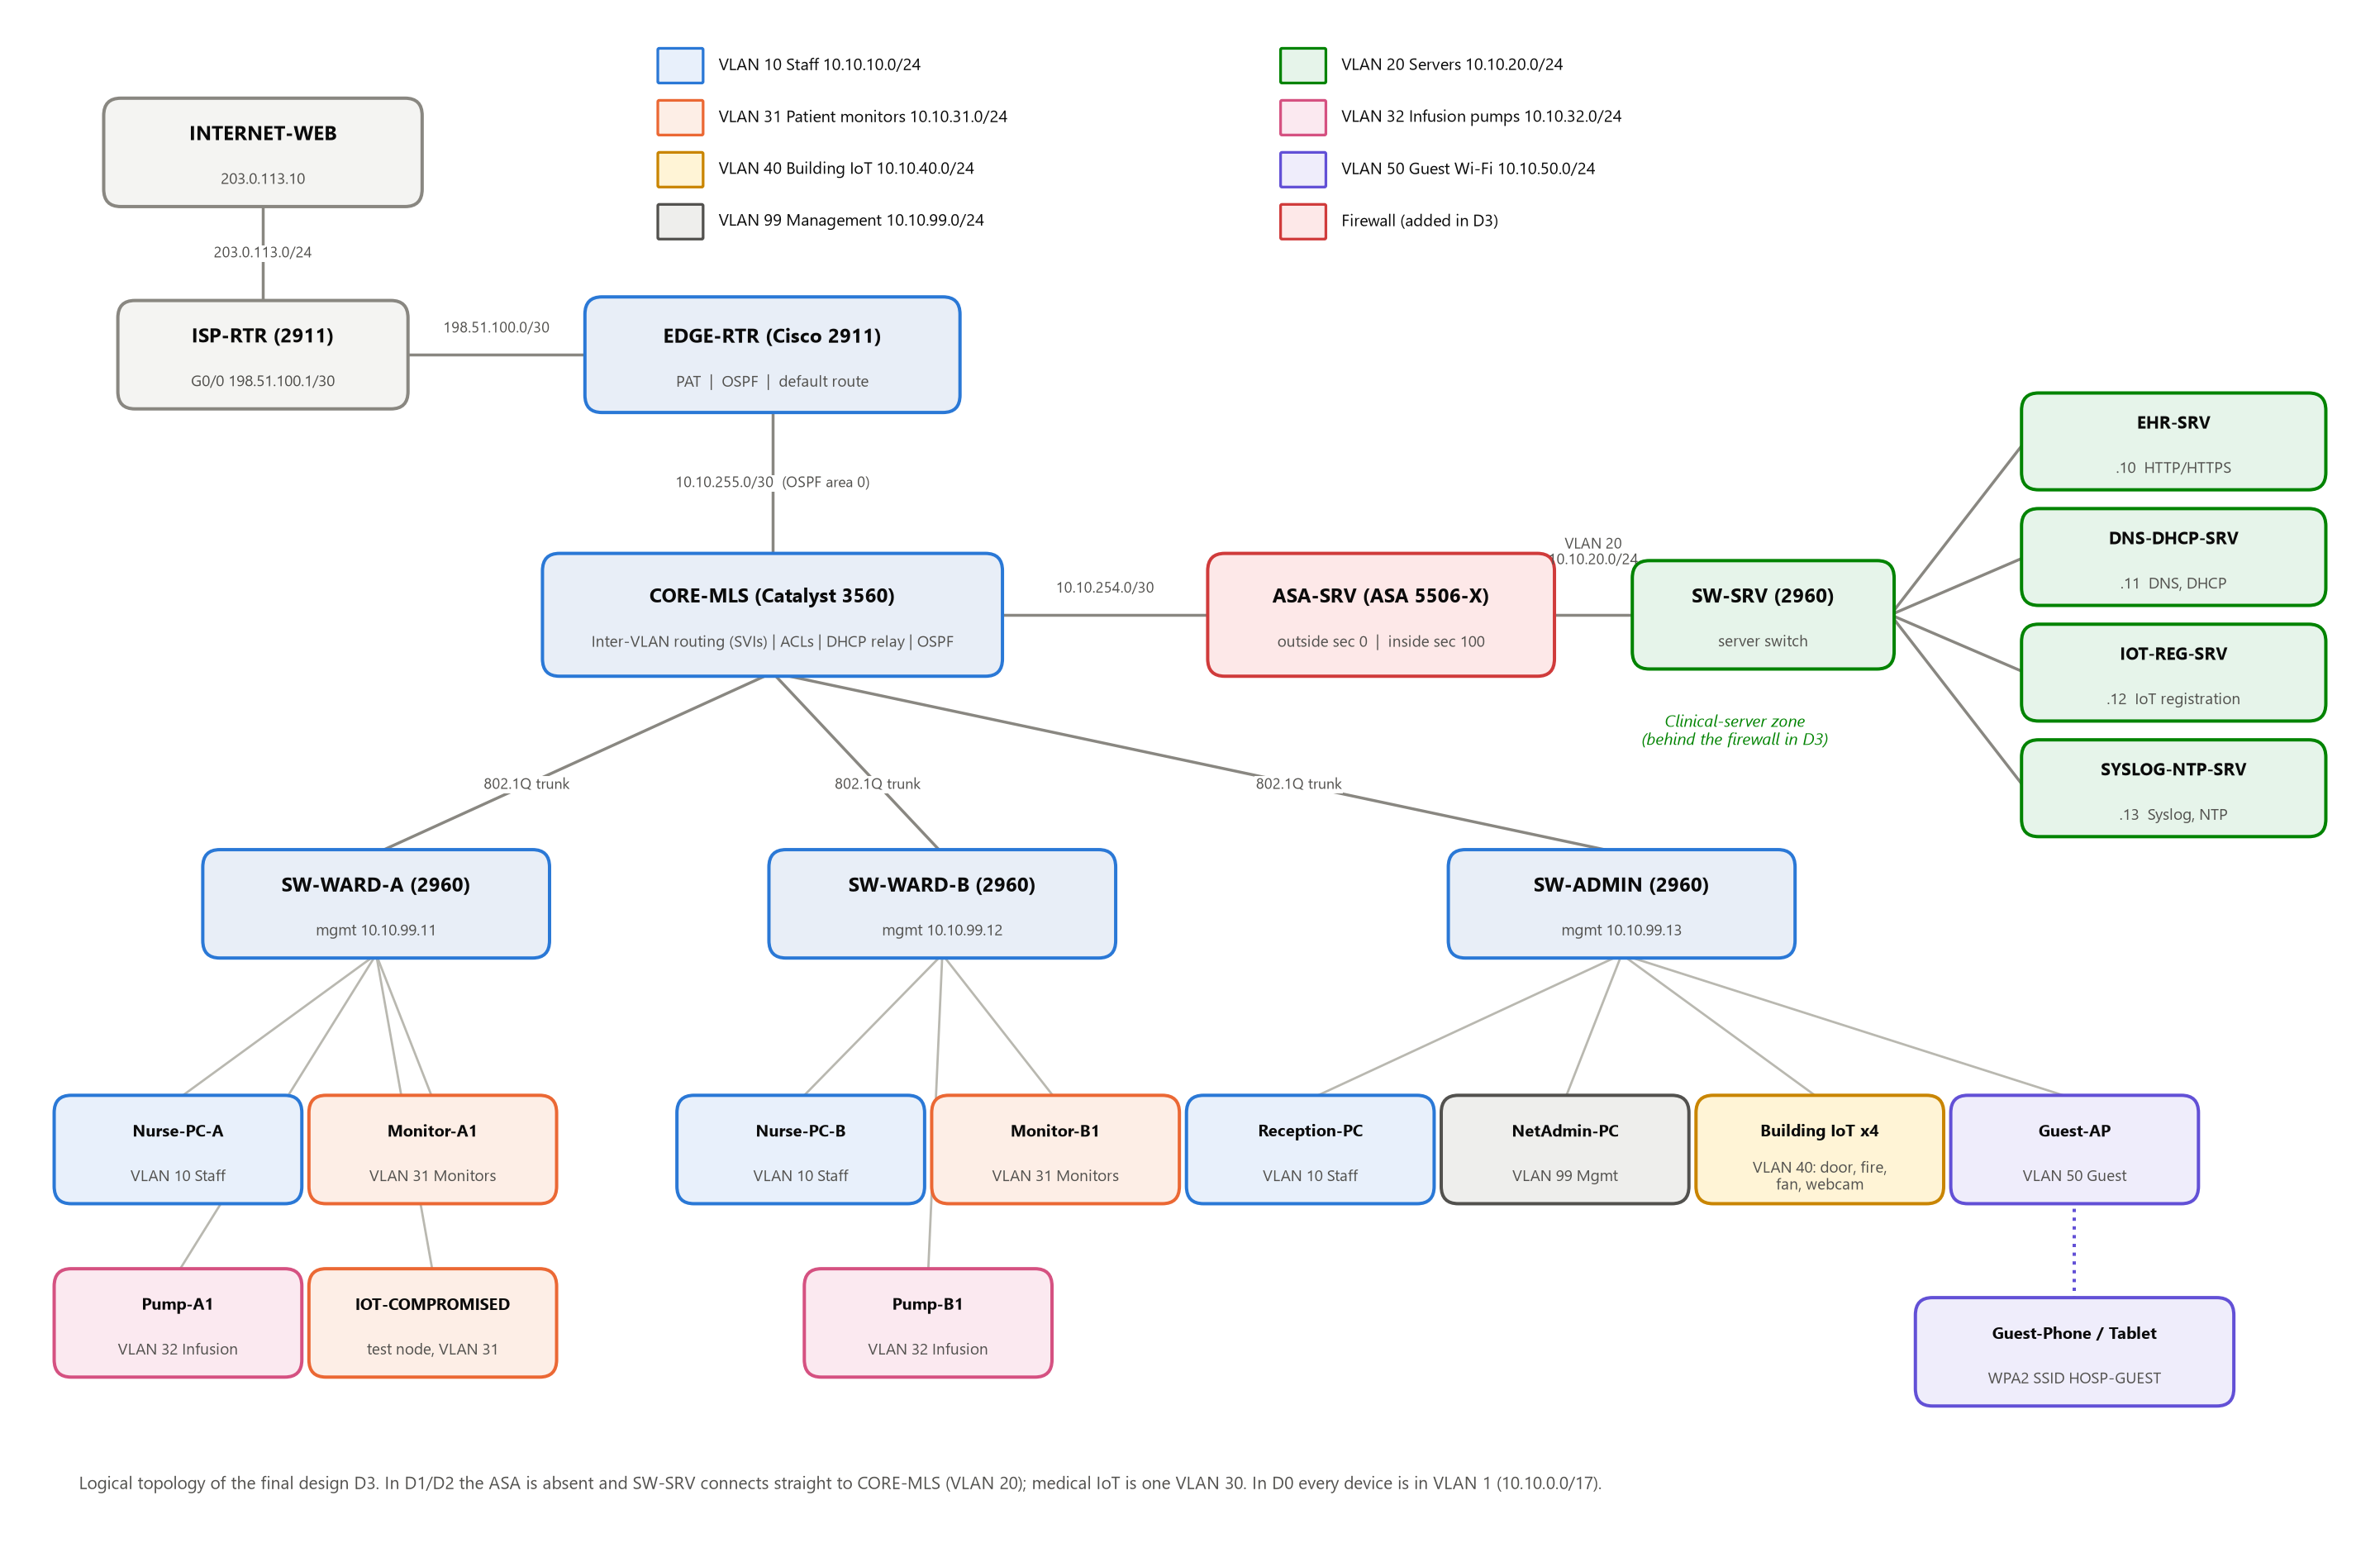
\includegraphics[width=0.88\textwidth]{topology.png}
\caption{Logical topology of D3. In D1/D2 the ASA is absent, SW-SRV attaches to CORE-MLS in VLAN~20 and all medical IoT shares VLAN~30. In D0 every device is in VLAN~1 (10.10.0.0/17). IOT-COMPROMISED is the test node at location L1.}
\label{fig:topology}
\end{figure*}

% AUTO-GENERATED by paper/gen_tables.py -- do not edit by hand; edit the data and re-run.
\begin{table}[t]
\centering
\caption{VLAN and addressing plan extracted from the configurations (10.10.\textit{VLAN}.0/24, gateway .1).}
\label{tab:vlans}
\scriptsize
\setlength{\tabcolsep}{3pt}
\begin{tabular}{@{}rllll@{}}
\toprule
VLAN & Name & Subnet & Designs & Members \\
\midrule
1 & default (flat) & 10.10.0.0/17 & D0 & Every device (flat) \\
10 & STAFF & 10.10.10.0/24 & D1--D3 & Nurse PCs, reception PC \\
20 & SERVERS & 10.10.20.0/24 & D1--D3 & EHR, DNS/DHCP, IoT reg., Syslog/NTP \\
30 & MED-IOT & 10.10.30.0/24 & D1--D2 & All medical IoT \\
31 & MED-MONITORS & 10.10.31.0/24 & D3 & Patient monitors \\
32 & MED-INFUSION & 10.10.32.0/24 & D3 & Infusion pumps \\
40 & BLDG-IOT & 10.10.40.0/24 & D1--D3 & Door, fire monitor, fan, webcam \\
50 & GUEST & 10.10.50.0/24 & D1--D3 & Guest Wi-Fi clients \\
99 & MGMT & 10.10.99.0/24 & D1--D3 & Switch mgmt, NetAdmin-PC \\
998 & NATIVE-UNUSED & -- & D3 & Unused native VLAN on trunks \\
999 & BLACKHOLE & -- & D3 & Parked (shut) ports \\
\bottomrule
\end{tabular}
\end{table}


\subsection{Designs}
\label{sec:designs}
The four designs share devices, cabling, servers and end-device settings. The one exception is that D3 inserts an ASA~5506-X between CORE-MLS and SW-SRV. Otherwise only the device configurations change.

\textbf{D0 Flat:} one broadcast domain (10.10.0.0/17) and Telnet management with a shared password.
\textbf{D1 VLAN-only:} six role VLANs (staff 10, servers 20, medical IoT 30, building IoT 40, guest 50, management 99), routed by CORE-MLS without filtering.
\textbf{D2 Zone ACLs:} D1 plus inbound ACLs on SVIs 30, 40 and 50. IoT may reach the server subnet on any port, and guests may reach only DHCP, DNS and the Internet (Table~\ref{tab:acl}). Staff and management stay unfiltered.
\textbf{D3 Micro-segmentation:} monitors (VLAN~31) and pumps (VLAN~32) are split, and every IoT ACL has one service permit, TCP~80 to the registration server. ICMP echo-replies towards VLAN~99 are also permitted, so administrators can ping devices that cannot start a ping themselves. The server subnet moves behind the ASA. Its \cfg{OUTSIDE-IN} policy (\aceAsaDthree{} ACEs) repeats every permit statefully~\cite{ciscoasa922}; for example, only 10.10.10.0/24 reaches the EHR. Every access port runs sticky port security with \cfg{violation shutdown}, PortFast and BPDU Guard. DHCP snooping trusts only the uplinks~\cite{rfc3046}. Trunks use native VLAN~998, explicit allowed lists and \cfg{nonegotiate}, and unused ports are shut in VLAN~999. Management is SSHv2 only~\cite{rfc4253}, from VLAN~99 only (\cfg{access-class 10 in}).

% AUTO-GENERATED by paper/gen_tables.py -- do not edit by hand; edit the data and re-run.
\begin{table}[t]
\centering
\caption{Key ACL lines, verbatim from the configuration files (``!'' lines added as labels). D2's zone permit admits the whole server subnet, so the F-1 and H-1 denies must carve out router addresses; D3 permits one host and one port.}
\label{tab:acl}
\scriptsize
\begin{minipage}{\columnwidth}
\begin{verbatim}
! D2 CORE-MLS: coarse zone ACL, SVI 30 (inbound)
ip access-list extended MEDIOT-IN
 permit udp any host 255.255.255.255 eq 67
 permit udp any host 10.10.20.11 eq 67
! F-1: exclude the core's own SVI-20 address
 deny ip any host 10.10.20.1
 permit ip 10.10.30.0 0.0.0.255 10.10.20.0 0.0.0.255
 deny ip any any
! D2 GUEST-IN (deny lines only)
! H-1: exclude EDGE-RTR's WAN /30
 deny ip any 198.51.100.0 0.0.0.3
 deny ip any 10.0.0.0 0.255.255.255
! D3 CORE-MLS: least privilege, SVI 31 (inbound)
ip access-list extended MONITORS-IN
 permit udp any host 255.255.255.255 eq 67
 permit udp any host 10.10.20.11 eq 67
 permit tcp 10.10.31.0 0.0.0.255 host 10.10.20.12 eq 80
 permit icmp 10.10.31.0 0.0.0.255 10.10.99.0 0.0.0.255 echo-reply
 deny ip any any
! D3 ASA-SRV access-list OUTSIDE-IN extended (excerpt)
 permit tcp 10.10.10.0 255.255.255.0 host 10.10.20.10 eq 80
 permit tcp 10.10.31.0 255.255.255.0 host 10.10.20.12 eq 80
 deny ip any any
\end{verbatim}
\end{minipage}
\end{table}


\subsection{Pre-deployment verification}
\label{sec:verify}
Before the designs were tested in the simulator, two independent checks reviewed the configurations. The first is a static reachability analyser (\texttt{tools/policy\_analyzer.py}) that reads only the configuration files and the end-device sheet. It models bridge domains, connected, static and OSPF routes, IOS and ASA ACLs with first-match semantics, ASA security levels and connection state, PAT, VTY rules, DHCP relay and snooping, and port security. It walks every test packet hop by hop and records the configuration line that decides it. A pytest suite (125 tests) checks the ACL engine and lints the configurations. It also mutates them, for example by removing an ACL layer or snooping trust, to confirm that a verdict flips. The second check is a third-party configuration-review checklist (ECC~2.2.3 \texttt{network-config-reviewer}), whose findings are recorded in the project's \texttt{tests/FINDINGS.md}. Findings were fixed in the configuration files, and the original files were archived so that both versions can be analysed (Section~\ref{sec:res-verify}).

\subsection{Threat model and test suite}
The adversary fully controls one IoT device and can send arbitrary IP traffic from its port and address. The adversary knows the addressing plan but holds no credentials and cannot exploit IOS or ASA software. Packet Tracer smart devices cannot originate attack traffic, so a laptop (IOT-COMPROMISED) takes the device's port, VLAN and DHCP lease. It is placed at L1, SW-WARD-A Fa0/4 (medical VLAN 30/31); at L2, SW-WARD-B Fa0/4; and at L3, SW-ADMIN Fa0/7 (building VLAN~40). Table~\ref{tab:attackdef} lists the tests and their nearest ATT\&CK techniques~\cite{mitreattack}. A1 probes a fixed inventory of 23 hosts and 10 services. The hosts are staff, servers, IoT, guests and five network-device addresses; the services are EHR HTTP/HTTPS, IoT HTTP, DNS, an Internet web server, and Telnet/SSH on five devices. A1--A4 run at L1--L3 and A5--A8 at fixed ports, three trials each. Nine functional tests (Table~\ref{tab:functional}) check that legitimate flows still work.

\begin{table}[t]
\centering
\caption{Tests and nearest MITRE ATT\&CK techniques.}
\label{tab:attackdef}
\scriptsize
\setlength{\tabcolsep}{2.5pt}
\begin{tabular}{@{}lp{0.56\columnwidth}p{0.30\columnwidth}@{}}
\toprule
ID & Procedure & ATT\&CK \\
\midrule
A1 & ICMP sweep of the 23-host inventory & T1018, T1046 \\
A2 & HTTP to the EHR (10.10.20.10) & T1213 \\
A3 & IoT-server login page; ping Pump-A1 (other class) & T1021 \\
A4 & Telnet/SSH to switch, gateway and router addresses & T1021.004 \\
A5 & Rogue DHCP server on a staff jack (SW-WARD-A Fa0/5) & T1557.003 \\
A6 & Laptop replaces Monitor-A1 on SW-WARD-A Fa0/2 & T1200 \\
A7 & Guest phone: HTTP to the EHR & T1213 \\
A8 & Rogue 2960 on a staff jack negotiates a trunk (DTP) & T1200, T1599 \\
Q1 & Detect node from ACL deny counters; move its port to VLAN~999 & (response) \\
O1 & 10-ping RTT and tracert hops for three legitimate flows & -- \\
\bottomrule
\end{tabular}
\end{table}

\subsection{Automated execution (ptlab)}
The stock Packet Tracer MCP bridge can only exchange ICMP between named devices. Our gateway, ptlab, patches Packet Tracer's script module with a generic evaluation hook (\texttt{ptEval}). On top of it, it adds 16 tools to the 18 stock ones: PC command output (ping, telnet, ssh, nslookup, tracert), a browser client, IOS \cfg{show} capture, and configuration of server services, DHCP pools and DNS records. These are served over a loopback REST API and an MCP proxy. A runner opens each design file and applies the GUI set-up checklist. It then runs A1--A8, Q1, O1 and the automatable functional tests (all except F3 and F8, which stay manual), and writes every observation with raw evidence to the result files. Q1 snapshots the deny counters of the node's SVI ACL while the node pings a management address. After three new denies it locates the node's port in the MAC address table and moves it to VLAN~999. It then records the time to detect and contain, and whether staff can still reach the EHR. Before and after each of A1--A4 the runner reads the CORE-MLS and ASA deny counters; a rise counts as a detection.

\subsection{Metrics}
An attack run is \emph{succeeded} (S) if it reaches every target in scope, \emph{partial} (P) if it reaches some, and \emph{blocked} (B) if it reaches none. Per design we report the majority over runs, with ties going to the outcome worse for the defender. Attack surface counts reachable hosts and services. The metrics follow the literature. Attack-surface reduction is $\mathrm{ASR}=1-\text{reachable}/23$, and the blast radius $\mathrm{BR}_w$ weights each reachable host by an asset-criticality score that we assign (1--5)~\cite{Odule2026SimulationValidation}. Attack block rate (ABR) is the share of blocked attempts. Policy-compliance rate (PCR) counts blocked unauthorised plus passed authorised checks~\cite{Mughaid2026SecureAdaptive}. Detection coverage is the share of attack windows with a deny-counter rise. Fisher's exact test compares blocked attempts between adjacent designs. Configuration cost counts the commands in all device files (excluding comments and mode wrappers), the ACEs, and the 12 security features detected by configuration pattern.
